\documentclass{article}
\usepackage[utf8]{inputenc}
\usepackage{longtable}
\usepackage{authblk}
\usepackage{adjustbox}
\usepackage{natbib}

\title{POBLACIÓN DE COLOMBIA}
% autor
\author[1]{\normalsize Mario Fernando Titua\~na De La Vega}
\affil[1]{\small  Escuela de Ingeniería,Universidad de los Andes\\
\texttt{{mf.tituana}@uniandes.edu.co}}
\date{30 de Junio de 2018}



\usepackage{Sweave}
\begin{document}
\Sconcordance{concordance:proyecto1.tex:proyecto1.Rnw:%
1 16 1 1 0 10 1 1 6 1 5 11 1 1 5 14 0 1 2 7 1 1 10 1 4 9 1 1 11 1 3 11 %
1 1 6 12 0 1 3 2 1 1 9 13 0 1 2 5 1 2 2 7 1 1 8 1 9 31 0 1 2 7 1 1 22 2 %
1 1 34 4 1 1 29 1 3 12 1}

\maketitle
\begin{abstract}

Este es mi primer trabajo en exploracion y modelamiento de indices usando LATEX.Este trabajo lo he hecho bajo la filosa de trabajo replicable. Este es mi primer trabajo en exploracion y modelamiento de indices usando LATEX. Este trabajo lo he hecho bajo la filosofa de trabajo replicable. Para ete trabajo se aplica varios datos de Colombia tiene una economía diversificada y posee un importante componente de servicios. La producción económica del país está dominada por su demanda interna y el gasto en consumo de los hogares es el mayor componente del PIB. El PIB en 2016 fue de 720 151 millones de dólares.El índice de desarrollo humano colombiano es de 0,727 y su esperanza de vida al nacer es de 74,8 años.Colombia es parte del grupo de los CIVETS considerados como seis principales mercados emergentes. Es miembro de la OCDE, la OEA, la Alianza del Pacífico, es el único país de América Latina que es socio global de la OTAN, y otras organizaciones internacionales. Es el tercer país más desigual en América Latina, después de Honduras y Haití; a nivel mundial Colombia es el noveno país más desigual del mundo. Para este trabajo se aplicara lo aprendido en clases, exploracion y modelamiento de indices usando LATEX. 
\end{abstract}
\section*{Introducción}

Aqui les presento mi investigacion sobre diversos indices sociales en el mundo. Colombia, oficialmente República de Colombia, es un país soberano situado en la región noroccidental de América del Sur, que se constituye en un estado unitario, social y democrático de derecho cuya forma de gobierno es presidencialista. Es una república organizada políticamente en 32 departamentos descentralizados y el Distrito capital de Bogotá, sede del gobierno nacional. Incluyendo la isla de Malpelo, el cayo Roncador y el banco Serrana, el país abarca una superficie de 1 141 748 km², por lo que es el vigesimosexto país más grande del mundo y el séptimo más grande de América. Reclama como mar territorial el área hasta las 12 millas náuticas de distancia,  manteniendo un diferendo limítrofe al respecto con Venezuela y Nicaragua. Limita al Oriente con Venezuela y Brasil, al Sur con Perú y Ecuador y al Noroccidente con Panamá; en cuanto a límites marítimos, colinda con Panamá, Costa Rica, Nicaragua, Honduras, Jamaica, Haití, República Dominicana y Venezuela en el mar Caribe, y con Panamá, Costa Rica y Ecuador en el océano Pacífico. El ejecutivo estará formado por el Presidente de la República, por los ministros de despacho y por los directores de departamentos administrativos, así como por los gobernadores, alcaldías, superintendencias, establecimientos públicos y empresas industriales o comerciales del Estado. a rama judicial la forman la Corte Constitucional, la Corte Suprema de Justicia, el Consejo de Estado, el Consejo Superior de Judicatura, la Fiscalía General de la Nación, los tribunales y jueces civiles y militares.


Comencemos viendo que hay en la sección \ref{univariada} en la pagina \pageref{univariada}.


\section{Exploracion Univariada}\label{univariada}

 A la vez, el Congreso también podrá ejercer determinadas funciones legislativas. La Constitución de 1991 diseñó un modelo de justicia altamente politizado, y el resultado ha sido la existencia de injerencias del ejecutivo en los nombramientos clave del ramo, especialmente en el del Fiscal general, en el que se concretaron enormes poderes discrecionales. La Constitución de 1991 reorganizó el sistema de justicia civil que teóricamente es independiente del ejecutivo y el legislativo. Pero los miembros del aparato judicial son objeto de acciones intimidatorias cuando se tratan casos relacionados con miembros de las Fuerzas Armadas, paramilitares, guerrilleros o narcotraficantes. El sistema de justicia civil incorpora la jurisdicción regional que procesa los crímenes relacionados con tráfico de narcóticos, terrorismo, secuestros, etc. En estos tribunales los jueces, los testimonios, los fiscales y los abogados quedan en el anonimato por razones de seguridad. Esta modalidad de impartir justicia ha recibido condenas desde grupos de defensa de los Derechos Humanos ya que vulnera las normas legales y los drechos de procesamiento. Según el Estatuto Legal de Justicia este tipo de tribunales tendrían que desaparecer en junio de 1999.

Para conocer el comportamiento de las variables se ha preparado la Tabla \ref{stats}, donde se describe la distribución de las modalidades de cada variable. Los números representan la situación de algun pais en ese indicador, donde el mayor valor nurerico es la mejor situación.


Como apreciamos en la Tabla \ref{stats}, los paises en la mejor situación son los menos. \cite {freitas_evaluation_2015}

% Table created by stargazer v.5.2.2 by Marek Hlavac, Harvard University. E-mail: hlavac at fas.harvard.edu
% Date and time: sáb., jun. 30, 2018 - 3:07:59 p.m.
\begin{table}[!htbp] \centering 
  \caption{Medidas estadisticas} 
  \label{stats} 
\begin{tabular}{@{\extracolsep{5pt}}lcccc} 
\\[-1.8ex]\hline 
\hline \\[-1.8ex] 
Statistic & \multicolumn{1}{c}{N} & \multicolumn{1}{c}{Median} & \multicolumn{1}{c}{Max} & \multicolumn{1}{c}{Min} \\ 
\hline \\[-1.8ex] 
IDH & 32 & 0.804 & 0.879 & 0.691 \\ 
Población.Cabecera & 32 & 717,197 & 10,070,801 & 13,090 \\ 
Población.Resto & 32 & 268,111.5 & 1,428,858 & 21,926 \\ 
\hline \\[-1.8ex] 
\end{tabular} 
\end{table} 
%% figure
La institución judicial sufre la influencia de los mandos militares que habían conseguido que se legislase que cualquier actuación realizada en acto de servicio se considerara dentro de la jurisdicción militar y fuese juzgada por tribunales militares\cite{lima_rational_2015}. La Corte Constitucional excluyó la posibilidad de que las violaciones de Derechos Humanos pudiesen ser consideradas en relación al servicio militar y se habían de juzgar por tribunales civiles \cite{macqueen_methods_nodate}. Pero se han dado casos de violaciones de Derechos Humanos por parte de militares que han sido juzgadas por tribunales militares. La impunidad de las Fuerzas Armadas en este sentido se deja sentir en la justicia colombiana. Como se puede ver en la figura \ref{hist}.

\begin{figure}[h]
\centering
%\begin{adjustbox}{width=7cm,height=7cm,clip,trim=1.5cm 0.5cm 0cm 1.5cm}

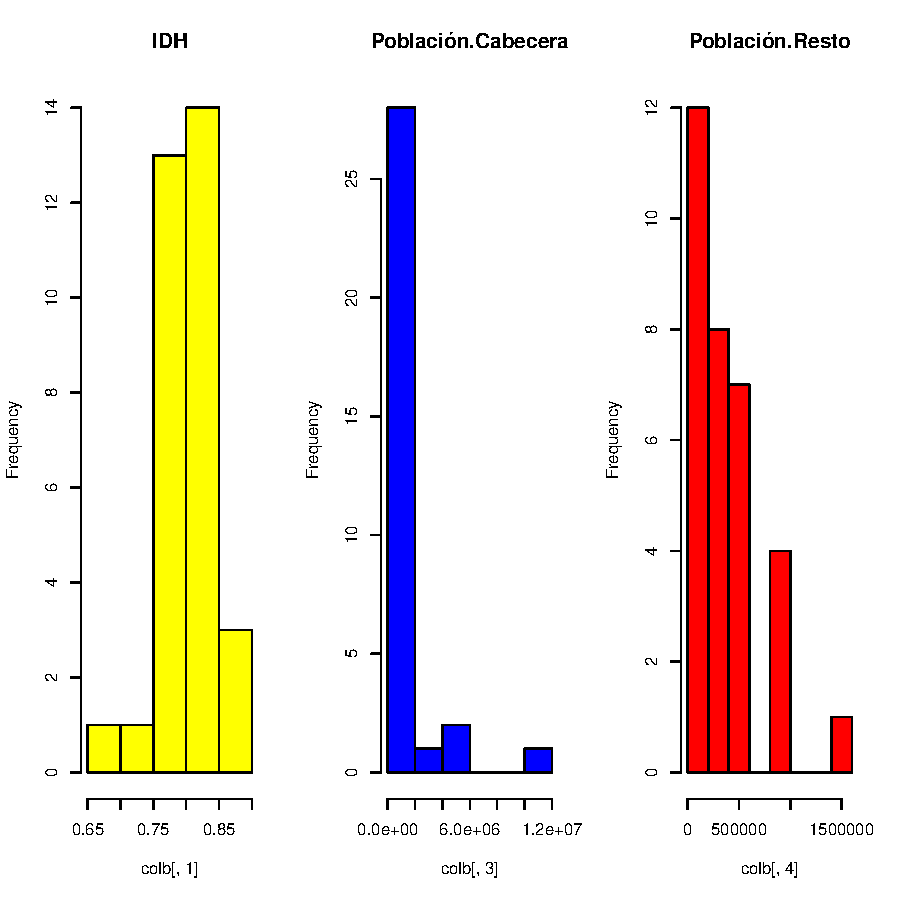
\includegraphics{proyecto1-barplots}
%\end{adjustbox}
\caption{Histogramas}
\label{hist}
\end{figure}
En 1991 se promulgó la nueva constitución en la que se desmantelaron todos los elementos del gobierno de coalición que existían desde 1974\cite{reynolds_clustering_2006}. La preparó una asamblea constituyente, designada por elección popular, en la que tuvieron una presencia importante representantes de un grupo de la guerrilla (la Alianza Democrática M-19) que se había desmovilizado (19 de los 70 constituyentes pertenecían a esta formación, junto con 24 representantes liberales y 20 conservadores), pero en la que tuvieron presencia otros grupos guerrilleros desmovilizados entre los que figuraba el grupo indigenista Comando Quintín Lamé, un sector del EPL (Ejército Popular de Liberación), el PRT (Partido Revolucionario de los Trabajadores), etc.Como se ve en la figura \ref{histor}.


\begin{figure}[h]
\centering
%\begin{adjustbox}{width=7cm,height=7cm,clip,trim=1.5cm 0.5cm 0cm 1.5cm}
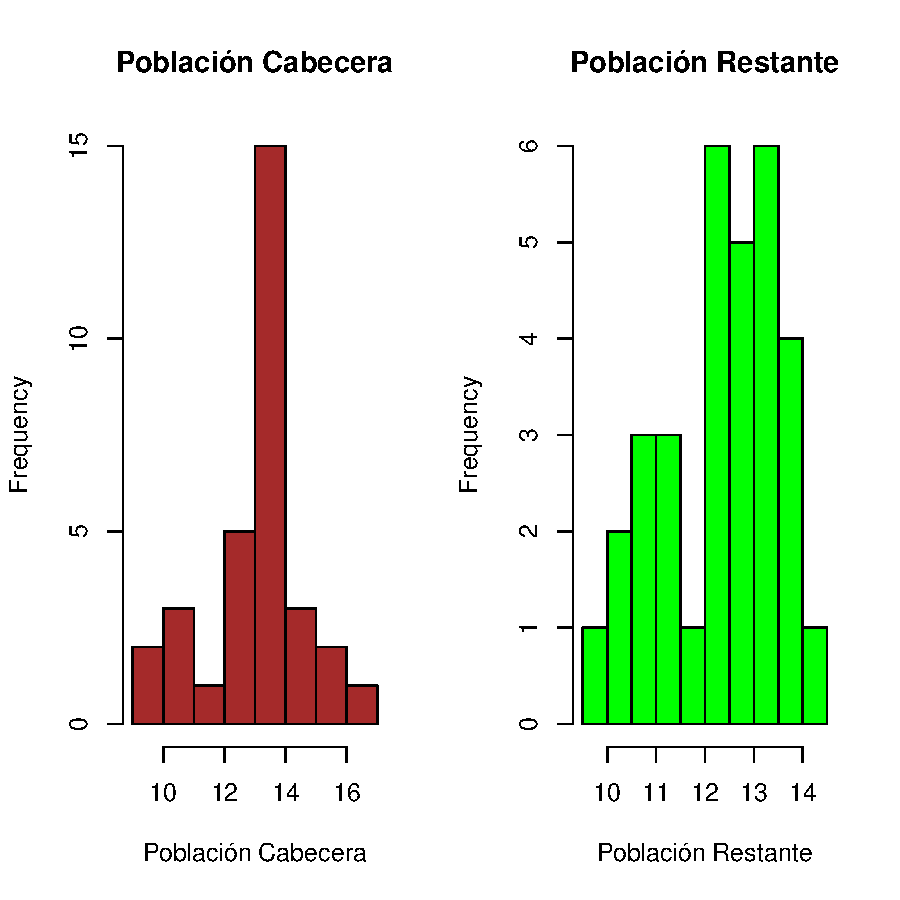
\includegraphics{proyecto1-histnorm}
%\end{adjustbox}
\caption{Histogramas Normalizados}
\label{histor}
\end{figure}

La reforma abarcaba la financiación estatal de las campañas por la Presidencia y el Congreso (hasta ese momento la financiación no era estatal y eso implicaba la existencia de inyecciones de dinero por parte de sectores interesados y el mantenimiento del clientelismo y la corrupción), la substitución de la Contraloría General por un tribunal nacional de cuentas y la independencia de la Defensoría del Pueblo de la Procuradoría General de la Nación. También se hacía referencia a la obligatoriedad del voto en las presidenciales del 98 y del 2002, la eliminación de la vicepresidencia, y la unificación y ampliación a cuatro años del mandato de alcaldes, gobernadores y regidores\cite{gower_general_1971}. Se propuso la eliminación de las incompatibilidades para congresistas y el aumento de las inhabilidades entre alcaldes y gobernadores, así como la unificación del calendario electoral. También se propuso una reducción de las atribuciones de la Corte Constitucional, que no podría pronunciarse sobre la constitucionalidad de los estados de excepción declarados por el ejecutivo. 


\section{Exploración Bivariada}

En este trabajo estamos interesados en el impacto de los otros indices en el nivel de Democracia. Veamos las relaciones bivariadas que tiene esta variable que se indica en la tabla \ref{corrDem}.El sistema de partidos actual está directamente relacionado con los acontecimientos y las dinámicas derivadas del período del Frente Nacional. En Colombia los partidos tradicionales pudieron mantener su posición hegemónica, debido a la falta de oposición obrera y de un partido centrista con arraigo electoral. Así, para los partidos colombianos fue más fácil integrar movimientos nuevos y unirse en una estrategia común para frenar el crecimiento de los partidos de izquierda y de partidos populistas independientes\cite{lima_rational_2015}.

% Table created by stargazer v.5.2.2 by Marek Hlavac, Harvard University. E-mail: hlavac at fas.harvard.edu
% Date and time: sáb., jun. 30, 2018 - 3:07:59 p.m.
\begin{table}[!htbp] \centering 
  \caption{Correlación de Democracia con las demás variables} 
  \label{corrDem} 
\begin{tabular}{@{\extracolsep{5pt}} cc} 
\\[-1.8ex]\hline 
\hline \\[-1.8ex] 
cabeLog & restoLog \\ 
\hline \\[-1.8ex] 
$0.487$ & $0.177$ \\ 
\hline \\[-1.8ex] 
\end{tabular} 
\end{table} Se indica la correlación entre las variables independientes en la siguiente tabla \ref{corrTableX}


% Table created by stargazer v.5.2.2 by Marek Hlavac, Harvard University. E-mail: hlavac at fas.harvard.edu
% Date and time: sáb., jun. 30, 2018 - 3:07:59 p.m.
\begin{table}[!htbp] \centering 
  \caption{Correlación entre variables independientes} 
  \label{corrTableX} 
\begin{tabular}{@{\extracolsep{5pt}} ccc} 
\\[-1.8ex]\hline 
\hline \\[-1.8ex] 
 & cabeLog & restoLog \\ 
\hline \\[-1.8ex] 
cabeLog & 1 &  \\ 
restoLog & 0.84 & 1 \\ 
\hline \\[-1.8ex] 
\end{tabular} 
\end{table} La organización del partido es débil y gira en torno a los respectivos líderes. Las pautas de autoridad entre patrones y clientes caracterizan desde hace mucho tiempo los partidos latinoamericanos, especialmente en Brasil y Colombia, donde los ‘coroneis’ y los ‘gamonales’ ejercían, respectivamente, su dominio en las zonas rurales y eran el vínculo crucial entre los líderes de los partidos y los votantes \cite{macqueen_methods_nodate}. De esta manera se resalta la existencia de relaciones clientelares, que se traducen en la compra de votos de los electores a cambio de favores individuales o colectivos. Estas relaciones clientelares se ven favorecidas por el mantenimiento de la estructura de la que forman parte los gamonales que se aprecia en la siguiente figura \ref{corrPlotX}
El clientelismo (un factor importante en el funcionamiento del sistema político), la crisis de los partidos tradicionals, la ineficacia administrativa, el exclusismo político, el retraso de la modernización política crearon un clima de desconfianza en el régimen político y de aquí se derivó una profunda crisis de legitimidad del sistema político (Gobierno, Congreso, corporaciones públicas) pero también existe una crisis de credibilidad hacia las Fuerzas Armadas, la justicia y los organismos de control del Estado.
Respecto a la Iglesia, se ha de decir que la iglesia católica colombiana ha sido una de las más ortodoxas, conservadoras y poderosas de las iglesias latinoamericanas. A finales de los años 80, la iglesia tenía gran influencia dentro del Partido Social Conservador y mantenía estrechas relaciones con diferentes gremios como la Unión de Trabajadores Colombianos y la Federación Agraria Nacional. Además la iglesia tiene un papel importante en dos ámbitos sociales concretos: el de la educación y el de las activitades de beneficencia. La iglesia es un actor político con peso dentro de las decisiones políticas estatales, debido a la vinculación de la jerarquía católica con las clases altas y medias de la sociedad colombiana. La participación de la iglesia en la vida política se manifesta en los procesos de pacificación y diálogo entre el Estado y los diferentes grupos guerrilleros.
\begin{figure}[h]
\centering
\begin{adjustbox}{width=10cm,height=7cm}
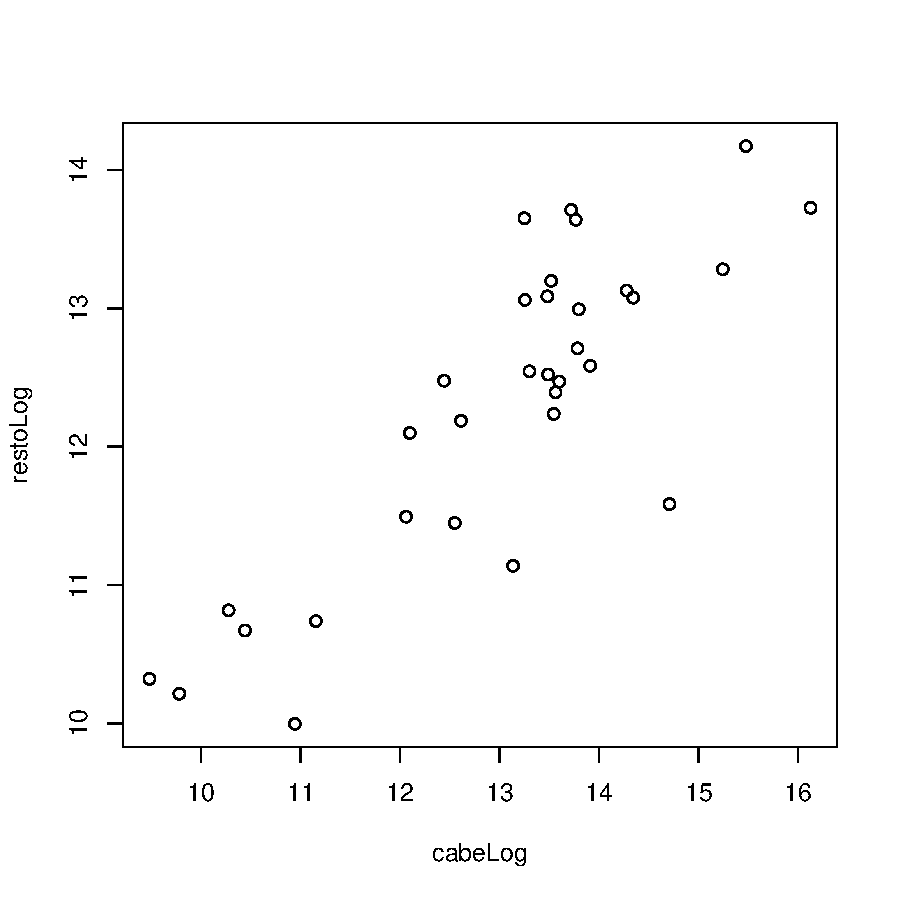
\includegraphics{proyecto1-corrPlotX}
\end{adjustbox}
\caption{correlación entre predictores}
\label{corrPlotX}
\end{figure}
 El sistema de gobierno colombiano se caracteriza por ser presidencialista, al igual que el resto de gobiernos de región. El presidencialismo colombiano ha generado una concentración del poder en manos del ejecutivoque queda reafirmada con la Constitución de 1991. El presidente de la república es el jefe de estado, de gobierno y suprema autoridad administrativa tal y como indica la Constitución de 1991 y se elige por voto directo y secreto de todos los/ciudadanos/as del país por un período de cuatro años sin posibilidad de ser reelegido. En caso de que ninguno de los candidatos consiga mayoría absoluta en la primera votación se llevará a cabo una segunda tres semanas después en la que participarán los dos candidatos más votados, el elegido será aquel que más votos obtenga. 
\section{Modelos de Regresión}

La expansión del papel de los militares está ligada estrechamente al fenómeno rural y político de ‘la violència’. Al desaparecer gradualmente este enfrentamiento, surgió uno nuevo: la guerra de guerrillas. Así que el ejército siemre ha estado dividido en unidades pequeñas y disperso por el país, patrullando y rastreando por las zonas inseguras, rebeldes y hostiles. Acostumbrado a la guerra antisubversiva, compuesto por pequeños destacamentos, no ha sido el tipo de ejército que organiza golpes de Estado. Sin embargo, las Fuerzas Armadas colombianas, al menos a nivel local, ejercen cierta influencia ya que sus cuadros de mando subsisten con frecuencia a una administración civil que parece incapaz de cumplir con sus tareas \cite{lima_rational_2015}. Las Fuerzas Armadas van aumentando su poder debido básicamente a la situación casi permanente de estado de sitio en la que ha vivido el país desde los tiempos del Frente Nacional. Los decretos 717 y 900 de 1997 con los que se crearon las zonas especiales de orden público en las que los militares y la policía pueden restringir los derechos de circulación y residencia, así como realizar violaciones de domicilio y rupturas sin orden como se aprecia en la sigueinte tabla \ref{regresiones}

% Table created by stargazer v.5.2.2 by Marek Hlavac, Harvard University. E-mail: hlavac at fas.harvard.edu
% Date and time: sáb., jun. 30, 2018 - 3:07:59 p.m.
\begin{table}[!htbp] \centering 
  \caption{Modelos de Regresión} 
  \label{regresiones} 
\begin{tabular}{@{\extracolsep{5pt}}lcc} 
\\[-1.8ex]\hline 
\hline \\[-1.8ex] 
 & \multicolumn{2}{c}{\textit{Dependent variable:}} \\ 
\cline{2-3} 
\\[-1.8ex] & \multicolumn{2}{c}{IDH} \\ 
\\[-1.8ex] & (1) & (2)\\ 
\hline \\[-1.8ex] 
 cabeLog & 0.013$^{***}$ & 0.031$^{***}$ \\ 
  & (0.004) & (0.007) \\ 
  & & \\ 
 restoLog &  & $-$0.030$^{***}$ \\ 
  &  & (0.010) \\ 
  & & \\ 
 Constant & 0.634$^{***}$ & 0.766$^{***}$ \\ 
  & (0.055) & (0.065) \\ 
  & & \\ 
\hline \\[-1.8ex] 
Observations & 32 & 32 \\ 
R$^{2}$ & 0.238 & 0.425 \\ 
Adjusted R$^{2}$ & 0.212 & 0.385 \\ 
Residual Std. Error & 0.037 (df = 30) & 0.033 (df = 29) \\ 
F Statistic & 9.347$^{***}$ (df = 1; 30) & 10.706$^{***}$ (df = 2; 29) \\ 
\hline 
\hline \\[-1.8ex] 
\textit{Note:}  & \multicolumn{2}{r}{$^{*}$p$<$0.1; $^{**}$p$<$0.05; $^{***}$p$<$0.01} \\ 
\end{tabular} 
\end{table} 
A su vez, las Fuerzas Armadas colombianas han sido tradicionalmente débiles, pobres y carentes de prestigio pero tienen una influencia determinada dentro del Estado. En Colombia, las Fuerzas Armadas colombianas se han diferenciado de otras del continente por el hecho de que durante casi medio siglo han estado ocupadas de forma constante en operaciones militares activas (contra la guerrilla, los paramilitares, o contra los dos).


\section{Exploración Espacial}

Existen precedentes de la violencia rural en Colombia en los años 50 y 60. Se podían distinguir al menos cuatro tipos de situaciones que generaban violencia rural \cite{macqueen_methods_nodate} . Al primero se le ha de dar el nombre de ‘la venganza de los hacendados’ contra los campesinos que antes habían ocupado latifundios o reivindicado terrenos desocupados e intentado lanzar un desafío a la dominación de la clase terrateniente se muestra en la figura \ref{clustmap}






\begin{figure}[h]
\centering
%\begin{adjustbox}
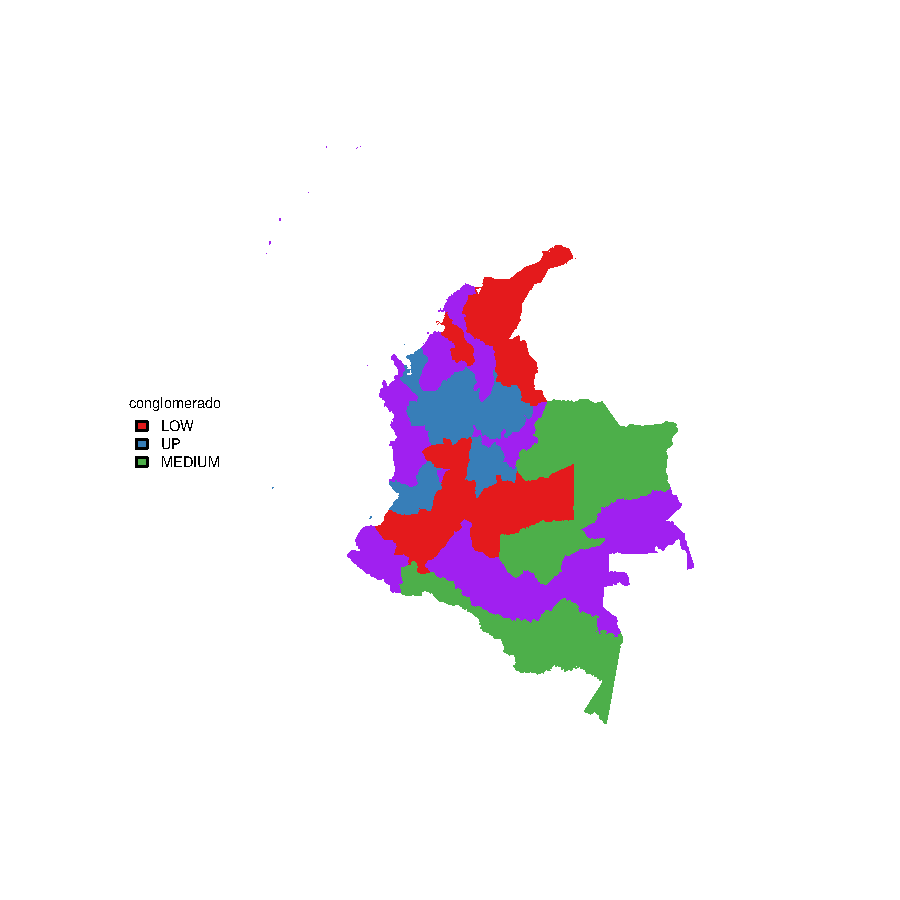
\includegraphics{proyecto1-plotMap1}
%\end{adjustbox}
\caption{Paises conglomerados segun sus indicadores sociopolticos}\label{clustmap}
\end{figure}
El segundo tipo, que era frecuente en las zonas donde existían propiedades medianas y pequeñas, estaba relacionado con las rivalidades entre familias y aldeas por la propiedad de la tierra y el control político. El tercer tipo se encontraba en las zonas donde los principales terratenientes y patrones habían huido, dejando a sus clientes en medio de disputas interminables e irresolubles por los recursos económicos y políticos. Finalmente, un cuarto tipo definido de forma menos clara ocurría cuando los hacendados liberales rebeldes reunían a sus trabajadores para atacar a las autoridades conservadoras y a sus aliados. Consecuencia frecuente de estas situaciones en el nivel local era la aparición del bandidaje y de las guerrillas partidistas. El resultado global era una guerra civil dentro de las clases y entre las clases \cite{gower_general_1971}. Después de diferentes gobiernos a principios de la década de los 60 era evidente la existencia de un problema en el campo colombiano que se caracterizó por una ininterrumpida, hasta el momento, guerra de guerrillas. 


%apalike apa
\bibliographystyle{abbrv}
\renewcommand{\refname}{Bibliografia}
\bibliography{Colombia}


\end{document}
